
\begin{frame}
  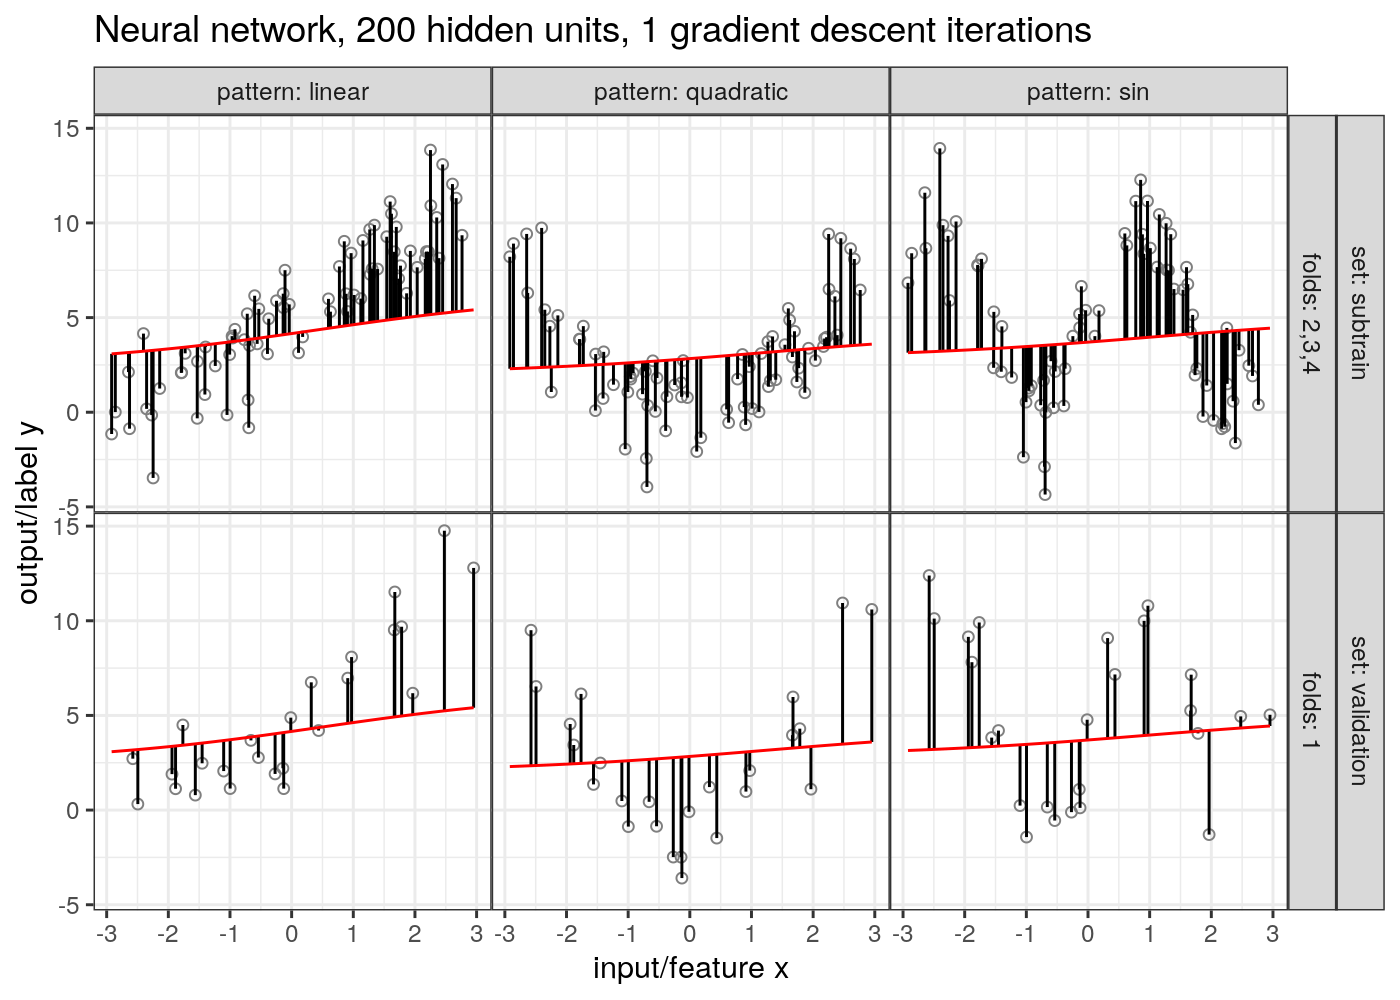
\includegraphics[width=\textwidth]{figure-overfitting-pred-units=200-maxit=1.png}
\
Data=grey dots, predictions=red curve, loss=black vertical line segments.
\end{frame}


\begin{frame}
  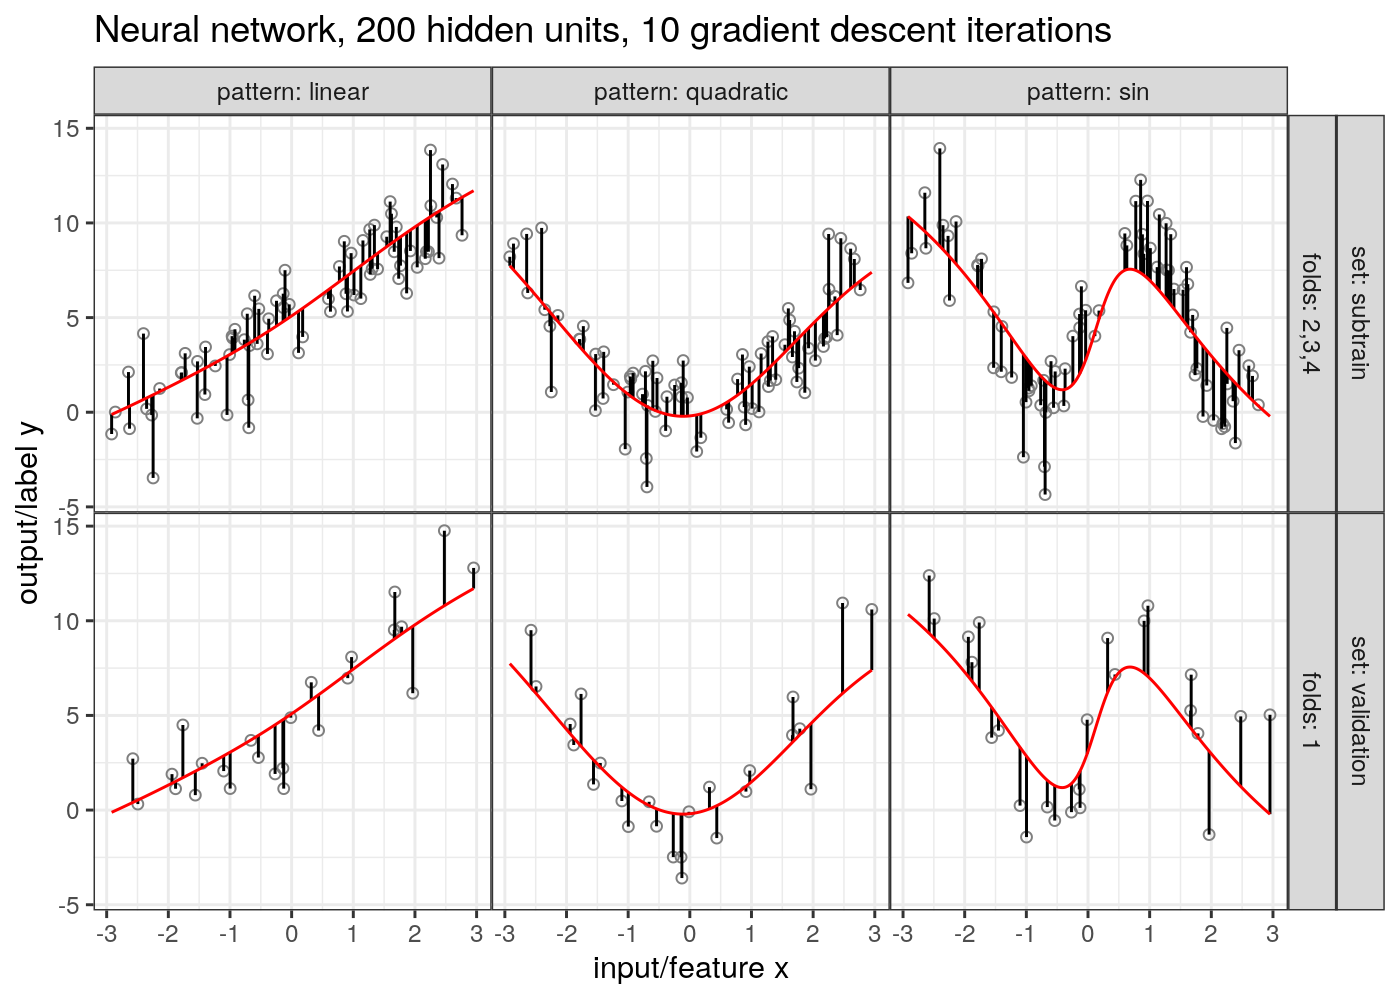
\includegraphics[width=\textwidth]{figure-overfitting-pred-units=200-maxit=10.png}
\
Data=grey dots, predictions=red curve, loss=black vertical line segments.
\end{frame}


\begin{frame}
  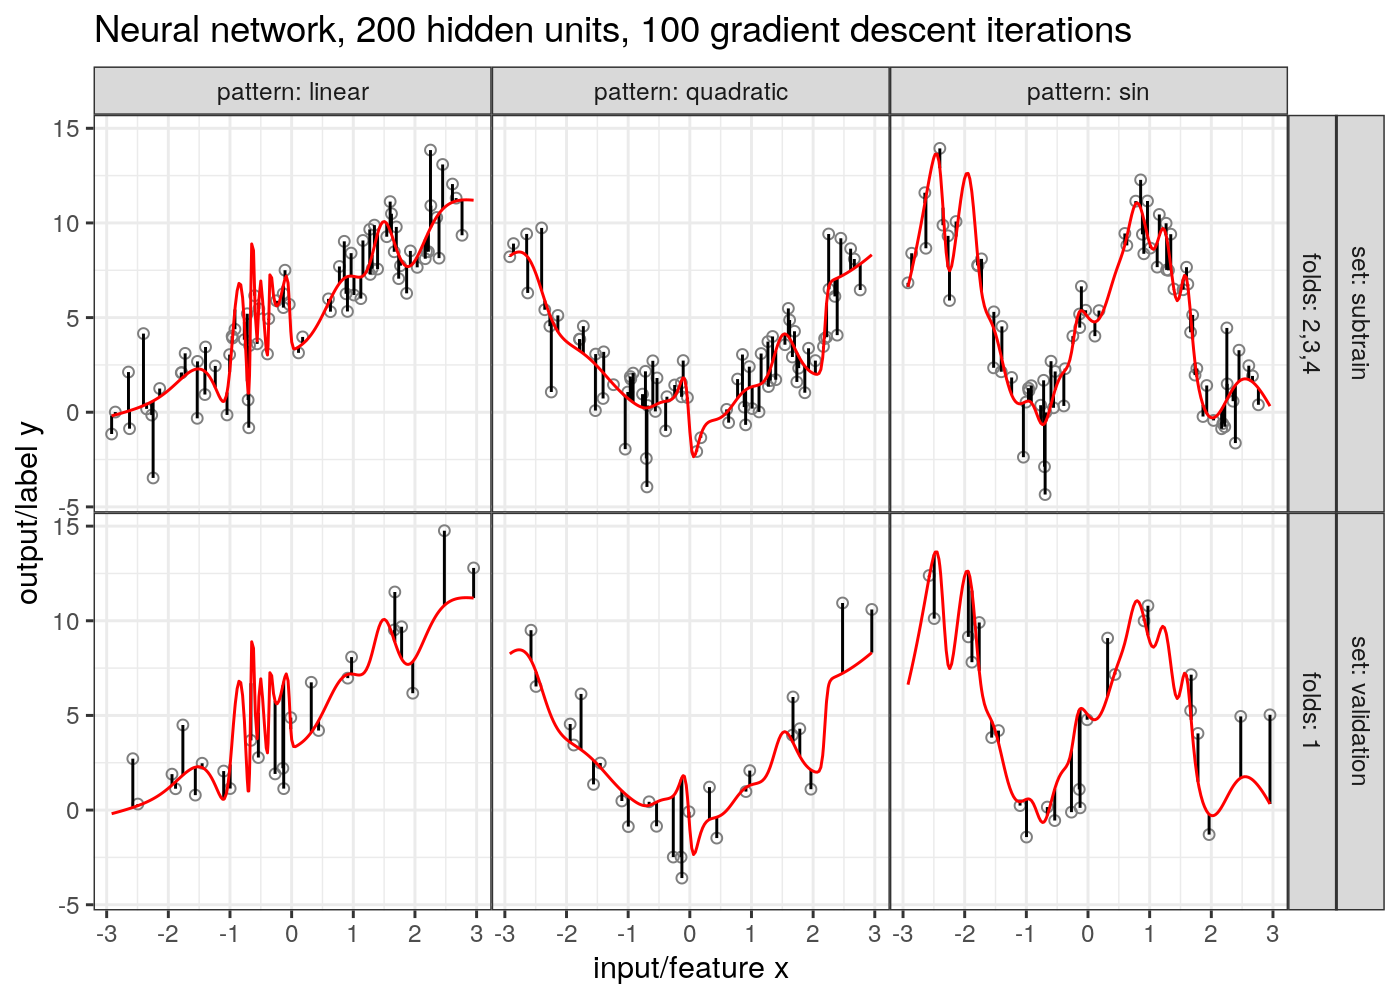
\includegraphics[width=\textwidth]{figure-overfitting-pred-units=200-maxit=100.png}
\
Data=grey dots, predictions=red curve, loss=black vertical line segments.
\end{frame}


\begin{frame}
  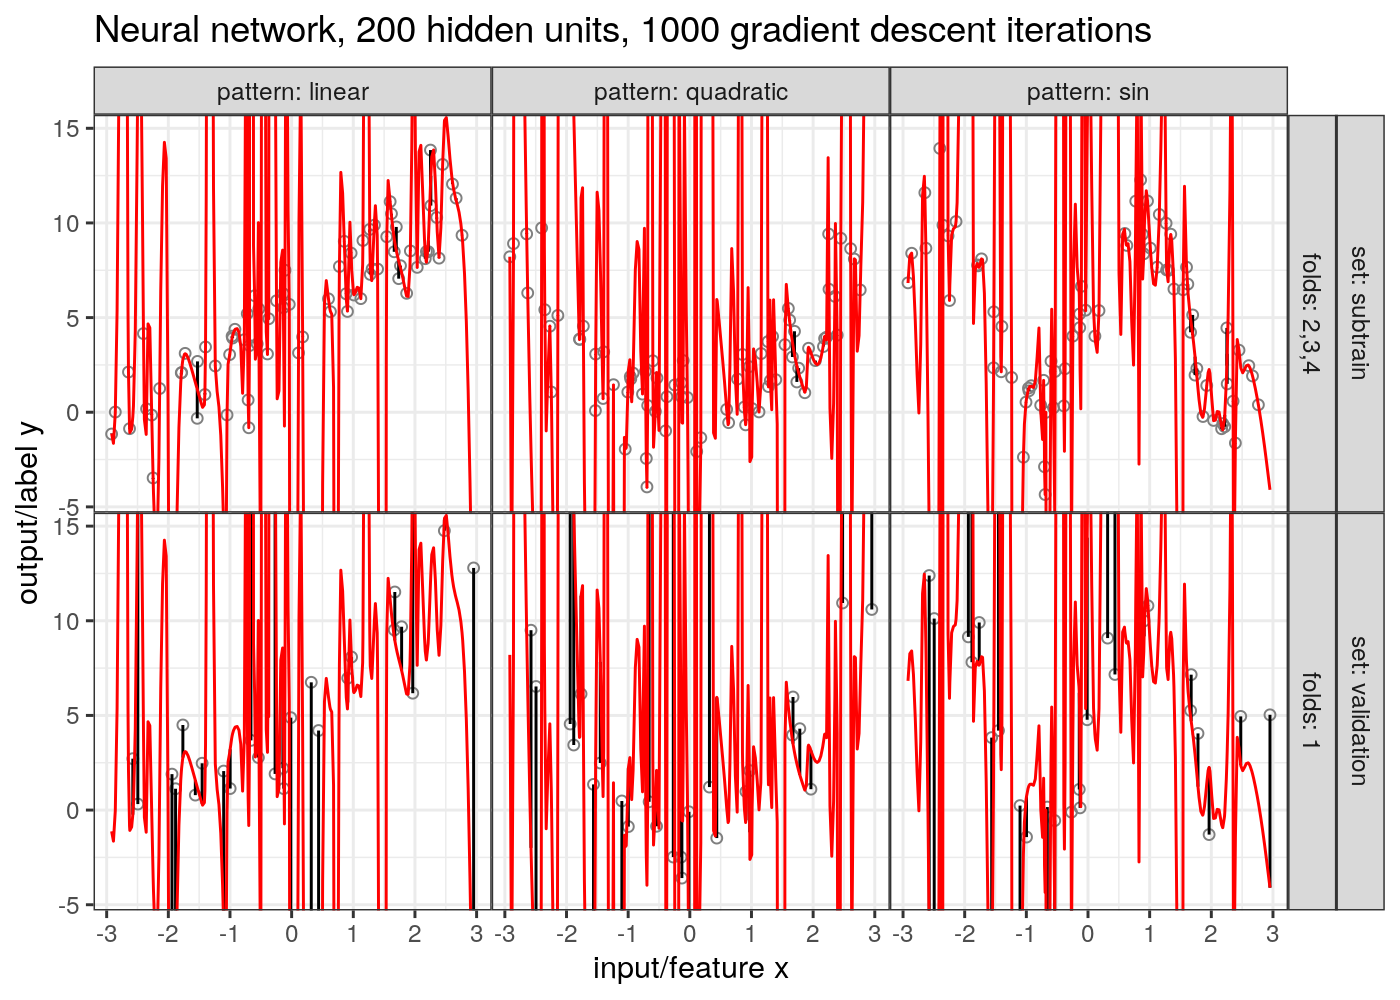
\includegraphics[width=\textwidth]{figure-overfitting-pred-units=200-maxit=1000.png}
\
Data=grey dots, predictions=red curve, loss=black vertical line segments.
\end{frame}


\begin{frame}
  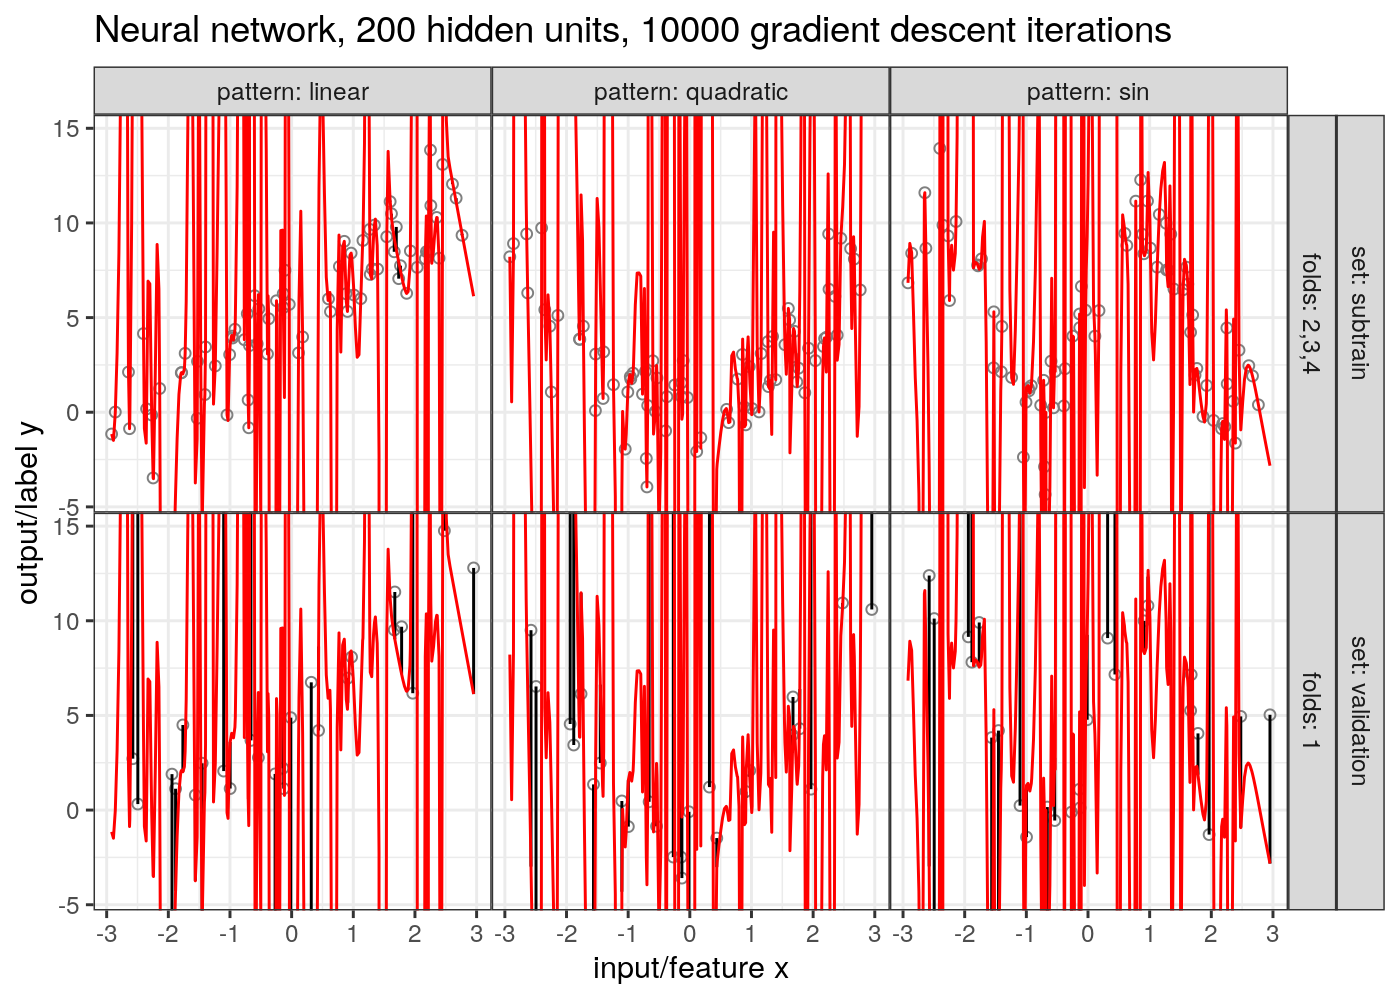
\includegraphics[width=\textwidth]{figure-overfitting-pred-units=200-maxit=10000.png}
\
Data=grey dots, predictions=red curve, loss=black vertical line segments.
\end{frame}


\begin{frame}
  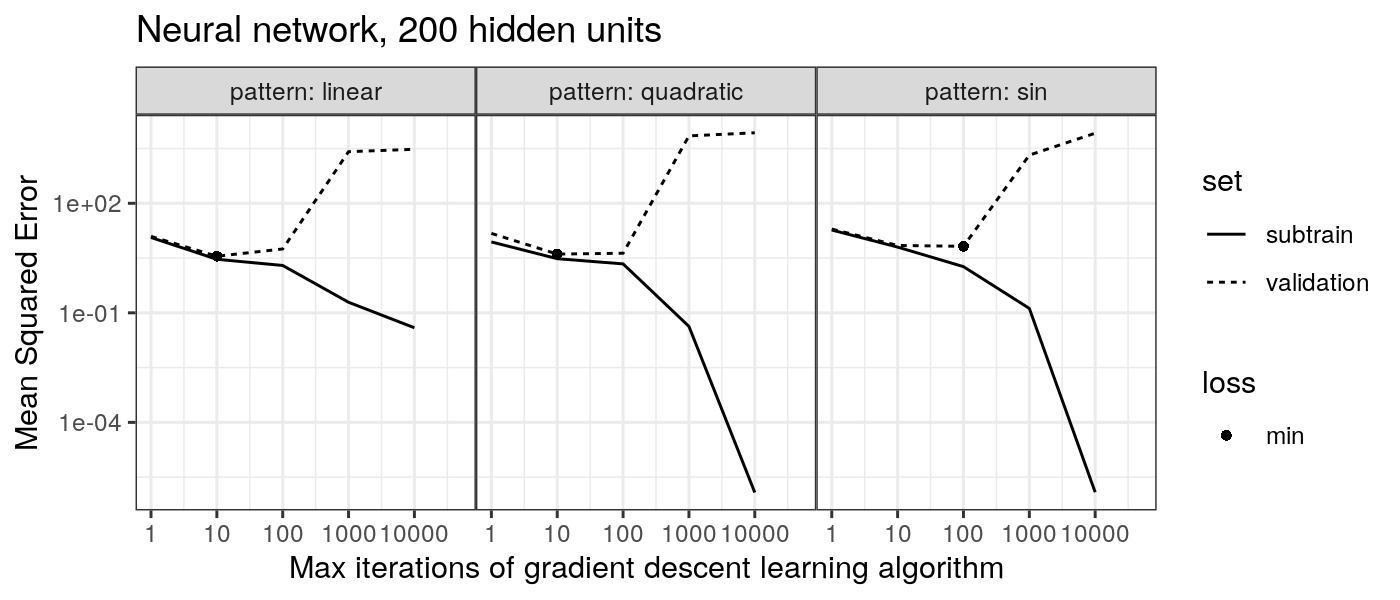
\includegraphics[width=\textwidth]{figure-overfitting-data-loss-200.png}
\
Data=grey dots, predictions=red curve, loss=black vertical line segments.
\end{frame}

